% !TEX TS-program = xelatex
% !TEX encoding = UTF-8 Unicode
% !Mode:: "TeX:UTF-8"

\documentclass{resume}
\usepackage{graphicx}
\usepackage{zh_CN-Adobefonts_external} % Simplified Chinese Support using external fonts (./fonts/zh_CN-Adobe/)
%\usepackage{zh_CN-Adobefonts_internal} % Simplified Chinese Support using system fonts
\usepackage{linespacing_fix} % disable extra space before next section
\usepackage{cite}
\usepackage{tabu}
\usepackage{multirow}
\usepackage{makecell}

\begin{document}
\pagenumbering{gobble} % suppress displaying page number
\pagestyle{empty}

% \name{严双林}
\large{
\renewcommand{\arraystretch}{1.2}
  \begin{tabu}{ c c r }
    &\multirow{5}{*}{\hspace{-12mm}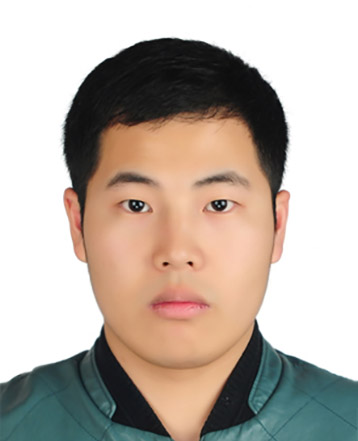
\includegraphics[width=0.88in]{ShuangLi.jpg}} \\
    \makecell[c]{\huge{\scshape{李爽}}} & \\
     ~~~~~~~~~~~~~~~~~~~~  男 | 重庆忠县 | 博士三年级研究生~~~~~~~~~~~~~~~~~~~ &  \\
     ~~~~~~~~~~~~~~~~~~~~ 重庆邮电大学 | 计算机科学与技术 | 人工智能与计算机视觉 ~~~~~~~~~~~~~~~~~~~~ &  \\
     ~~~~~~~~~~~~~~~~~~~~15870417922（微信同号） | shuangli936@gmail.com~~~~~~~~~~~~~~~~~~~~ &  \\
  \end{tabu}
}
% \large{
% \renewcommand{\arraystretch}{1.1}
%   \begin{tabu}{ c c l }
%    \multirow{4}{*}{\includegraphics[width=0.88in]{ShuanglinYan.jpg}}~~~~~~~~~~~& \multirow{4}{*}{\makecell[l]{\Huge{\textbf{严双林}}~~~~~~~~~~~~\\1997.06}} &  \\
%     &  & \email{shuanglinyan@njust.edu.cn} \\
%     &  & \phone{ (+86) 18487150593} \\
%     &  & \homepage[https://shuanglinyan.github.io]{https://shuanglinyan.github.io}\\
%     &  & \github[github.com/shuanglinyan]{https://github.com/shuanglinyan}\\
%   \end{tabu}
% }

% \basicInfo{
%   \email{shuanglinyan@njust.edu.cn} \textperiodcentered\ 
%   \phone{(+86) 184-871-50593} \textperiodcentered\ 
%   \homepage[https://shuanglinyan.github.io]{https://shuanglinyan.github.io} \textperiodcentered\ 
%   \github[github.com/shuanglinyan]{https://github.com/shuanglinyan}}
 
\section{\colorbox{gray}{\color{white}教育背景}}
\datedsubsection{\textbf{重庆邮电大学}, 重庆, 重庆}{2023.09 -- 至今}
计算机科学与技术学院, 计算机科学与技术工学博士\\
图像认知重庆市重点实验室, 导师: \href{https://scholar.google.com/citations?user=VZVTOOIAAAAJ&hl=zh-CN}{高新波教授}/\href{https://opentvi.github.io/team-ljx.html}{冷佳旭副教授}

\datedsubsection{\textbf{昆明理工大学}, 昆明, 云南}{2019.09 -- 2022.06}
信息工程与自动化学院, 计算机技术硕士\\
云南省人工智能重点实验室, 导师: \href{https://scholar.google.com.hk/citations?user=njjX8D0AAAAJ&hl=zh-CN}{李华锋教授}

\datedsubsection{\textbf{重庆邮电大学}, 重庆, 重庆}{2015.09 -- 2019.06}
计算机科学与技术学院, 软件工程学士\\
图像认知重庆市重点实验室, 本科导师: \href{https://faculty.cqupt.edu.cn/liulh/zh_CN/index.htm}{刘玲慧副教授}/\href{https://faculty.cqupt.edu.cn/luanxiao/zh_CN/index.htm}{栾晓教授}

% \section{\colorbox{gray}{\color{white}访学经历}}
% \datedsubsection{\textbf{香港理工大学}, 香港}{2025.06 -- 至今}
% 智慧健康中心, 访问学者, 合作导师: \href{https://research.polyu.edu.hk/en/persons/jing-qin}{秦璟教授}

% \datedsubsection{\textbf{新加坡科技设计大学}, 新加坡}{2023.09 -- 2024.09}
% 信息系统科技与设计系, 联合培养博士生, 合作导师: \href{https://scholar.google.com.hk/citations?user=Q5Ild8UAAAAJ&hl=zh-CN}{刘俊教授}
% % SUTD计算机视觉和学习实验室

% \datedsubsection{\textbf{京东探索研究院}, 北京}{2022.01 -- 2022.04}
% CV算法工程师, 合作导师: \href{https://scholar.google.com.hk/citations?hl=zh-CN&user=RwlJNLcAAAAJ}{陶大程院士} 
% 和 \href{https://scholar.google.com.hk/citations?hl=zh-CN&user=9jH5v74AAAAJ}{张敬博士}

\section{\colorbox{gray}{\color{white}研究兴趣}}
\textbf{多模态视觉智能}——跨模态表征学习，视觉-语言理解，视频智能分析

\textbf{开放场景视觉感知}——领域自适应，视频理解，目标检测，图像分割与图像增强

\section{\colorbox{gray}{\color{white}科研成果}}
围绕多模态视觉智能与跨模态表征学习开展研究，已在 IJCV、TIFS、TNNLS、TCSVT、PR 等国际权威期刊以及 ICML、AAAI、ACM MM 等 CCF-A 类会议发表论文10余篇，其中第一作者发表 ICML、TIFS、PR、TNNLS 等高水平论文。Google Scholar 引用数 = 677，H 指数 = 15（截至2026年8月）。更多信息请查看\href{https://scholar.google.com/citations?user=ePe0rG4AAAAJ&hl=zh-CN}{谷歌学术主页}。\\

\textbf{代表性学术论文:}
{\small 注：$^*$ 表示共同第一作者，$^\dagger$ 表示通讯作者。}
\begin{enumerate}[itemsep=1.8mm]

\item \textbf{Shuang Li}, Changjiang Kuang, Jiaxu Leng, Mingpi Tan, Zhanjie Wu, Shuanglin Yan, Xinbo Gao. Hyperbolic Hierarchical Alignment for Video-Based Visible-Infrared Person Re-Identification. {\textbf{ICML}}, 2026. (中国计算机学会推荐国际顶级学术会议 CCF-A 类)

\item \textbf{Shuang Li}, Jiaxu Leng, Changjiang Kuang, Mingpi Tan, Yu Yuan, Xinbo Gao. Causal Bootstrapped Alignment for Unsupervised Video-Based Visible-Infrared Person Re-Identification. {\textbf{TIFS}}, 2026. (SCI, 中科院一区 Top, 中国计算机学会推荐国际顶级学术期刊 CCF-A 类)



\item \textbf{Shuang Li}, Jiaxu Leng, Changjiang Kuang, Mingpi Tan, Xinbo Gao. Video-Level Language-Driven Video-Based Visible-Infrared Person Re-Identification. {\textbf{TIFS}}, 2025. (SCI, 中科院一区 Top, 中国计算机学会推荐国际顶级学术期刊 CCF-A 类)

\item \textbf{Shuang Li}, Jiaxu Leng, Ji Gan, Mengjingcheng Mo, Xinbo Gao. Shape-centered Representation Learning for Visible-Infrared Person Re-Identification. {\textbf{PR}}, 2025. (SCI，中科院一区 Top)

\item \textbf{Shuang Li}, Fan Li, Jinxin Li, Huafeng Li, Bob Zhang, Dapeng Tao, Xinbo Gao. Logical Relation Inference and Multiview Information Interaction for Domain Adaptation Person Re-Identification. {\textbf{TNNLS}}, 2023. (SCI，中科院一区 Top)



\item Yong Wu, Zijie Ding, Hongchao Li, Ze Zhou, Peng Hu, \textbf{Shuang Li$^\dagger$}. Dynamic Modality-Temporal Adaptation for Video-based Visible-Infrared Person Re-Identification. {\textbf{ACM MM}}, 2026. (中国计算机学会推荐国际顶级学术会议 CCF-A 类)
\end{enumerate}
\vspace{3mm}
\textbf{代表性合作研究成果:}

\begin{enumerate}[itemsep=1.8mm]
\item Yan Ding$^*$, \textbf{Shuang Li$^*$}, Huafeng Li, Guanqiu Qi, Baisen Cong, Yunpeng Gong, Zhiqin Zhu. Physical Regularization Loss: Integrating Physical Knowledge to Image Segmentation. {\textbf{IJCV}}, 2026. (中国计算机学会推荐国际顶级学术期刊 CCF-A 类)

\item Linhan Zhou$^*$, \textbf{Shuang Li$^*$}, Neng Dong, Yonghang Tai, Yafei Zhang, Huafeng Li. Hierarchical Prompt Learning for Image- and Text-Based Person Re-Identification. {\textbf{AAAI}}, 2026. (中国计算机学会推荐国际顶级学术会议 CCF-A 类)

% \item Sichen Tao$^*$, \textbf{Shuang Li$^*$}, Jun Ye, Neng Dong, Fan Li, Huafeng Li. Spatial-Temporal High-Frequency Learning for Video-based Visible-Infrared Person Re-Identification. {\textbf{TCSVT}}, 2026. (SCI，中科院一区 Top)

\item Yujie Yang$^*$, \textbf{Shuang Li$^*$}, Jun Ye, Neng Dong, Fan Li, Huafeng Li. DINOv2 Driven Gait Representation Learning for Video-Based Visible-Infrared Person Re-identification. {\textbf{ACM MM}}, 2025. (中国计算机学会推荐国际顶级学术会议 CCF-A 类)

% \item Zhiqin Zhu, Yang Yang, Guanqiu Qi$^\dagger$, \textbf{Shuang Li$^\dagger$}, Huafeng Li, Yu Liu$^\dagger$. Seeing Clearly, Detecting Precisely: Perceptual Enhancement and Focus Calibration for Small Object Detection. {\textbf{TNNLS}}, 2026. (SCI, 中科院一区 Top)

\item Jiaxu Leng, Zhengjie Wang, \textbf{Shuang Li$^\dagger$}, Xinbo Gao$^\dagger$. Dynamic-Static Collaboration for Unsupervised Domain Adaptive Video-Based Visible-Infrared Person Re-Identification. {\textbf{AAAI}}, 2026. (中国计算机学会推荐国际顶级学术会议 CCF-A 类)


% \item Yiming Wang, Guanqiu Qi, \textbf{Shuang Li$^\dagger$}, Yi Chai$^\dagger$, Huafeng Li. Body Part-Level Domain Alignment for Domain-Adaptive Person Re-Identification with Transformer Framework. {\textbf{TIFS}}, 2022. (SCI, 中科院一区 Top, 中国计算机学会推荐国际顶级学术期刊 CCF-A 类)


% \item Yafei Zhang, Yongzeng Wang, Huafeng Li$^\dagger$, \textbf{Shuang Li$^\dagger$}. Cross-Compatible Embedding and Semantic Consistent Feature Construction for Sketch Re-Identification. {\textbf{ACM MM}}, 2022. (中国计算机学会推荐国际顶级学术会议 CCF-A 类)


\end{enumerate}
\vspace{1mm}
% \textbf{发明专利:}
% \begin{enumerate}[itemsep=1.8mm]
% \item 基于判别字典学习和形态成分分解的多源图像融合方法. 李华锋, \textbf{严双林}, 王一棠, 余正涛, 王红斌. 专利号：ZL201810546687.7
% \end{enumerate}
\section{\colorbox{gray}{\color{white}项目经历与应用成果}}

\begin{enumerate}[itemsep=2.5mm]

\item \textbf{国家自然科学基金重点项目}
“面向跨设备多场景视频理解的可视分析技术研究”。


{\small
\textbf{项目成果：}“慧心极目·火眼金睛”视频监控系统；
\hspace{0.3cm} \textbf{承担角色：}核心技术负责人；\\
\textbf{贡献：}负责系统算法研发与建设，协同研究生开展视频感知、多模态理解与智能决策研究，支撑异常检测、行人检索等功能实现。
}


\item \textbf{重庆市重大专项}
“面向山地城市道路清扫场景的智慧环卫作业系统关键技术研发及应用”。

{\small
\textbf{项目成果：}Garden 智慧环卫大模型；
\hspace{2.5cm} \textbf{承担角色：}核心技术负责人；\\
\textbf{主要贡献：}负责 Garden 大模型数据体系建设，构建面向智慧环卫场景的视觉数据半自动循环标注与优化流程，为大模型训练提供高质量数据支撑。
}
\end{enumerate}


\section{\colorbox{gray}{\color{white}主持项目}}
\begin{enumerate}[itemsep=1.8mm]
\item 重庆市研究生科研创新项目“跨时间域行人重识别 - 鲁棒性信息深度挖掘研究”（项目编号：CYS25499），2024.07-2026-07，主持
\item 重庆邮电大学博士研究生创新人才项目“面向全天时跨模态多场景的行人重识别方法研究”（项目编号：BYJS202418），2024.12- 2026.12，主持
\end{enumerate}

\section{\colorbox{gray}{\color{white}学术服务}}
% \begin{itemize}[itemsep=1.8mm]
%   \item 担任 TIP、TIFS、TNNLS、TMM、TCSVT、TETCI、IoT、PR 等期刊审稿人
%   \item 担任 CVPR、ICCV、ECCV、ICLR、ICML、NeurIPS、AAAI、ACM MM、IJCAI、PRCV 等会议审稿人
% \end{itemize}
\begin{itemize}[itemsep=1mm]

  \item 担任 TIP、TIFS、TNNLS、TMM、TCSVT、PR、TETCI 等期刊审稿人
  \item 担任 CVPR、ICCV、ECCV、ICLR、ICML、NeurIPS、AAAI、ACM MM、IJCAI 等会议审稿人

\end{itemize}

\section{\colorbox{gray}{\color{white}荣誉与奖励}}
\begin{itemize}[itemsep=1.8mm]
  \item 重庆邮电大学博士研究生学业一等奖学金（三次），2023--2025
  \item 云南省优秀硕士学位论文, 2022
  \item 昆明理工大学优秀硕士学位论文, 2022
  \item 重庆邮电大学优秀本科毕业论文, 2019

\end{itemize}

% \textbf{国家留学基金委奖学金, 2023}
% \vspace{2mm}

% \textbf{南京理工大学学业奖学金, 2020-2023}
% \vspace{2mm}

% \textbf{昆明理工大学优秀毕业生, 2017}
% \vspace{2mm}

% \textbf{国家/云南省政府励志奖学金, 2015-2016}
% \vspace{2mm}

% \textbf{昆明理工大学优秀学生干部, 2015}

%% Reference
%\newpage
%\bibliographystyle{IEEETran}
%\bibliography{mycite}
\end{document}
